\documentclass[a4paper,10pt,oneside]{scrbook}

% input encoding
\usepackage[utf8]{inputenc}

% graphics support
\usepackage{graphicx}
\usepackage{float}

% math packages
\usepackage{amsmath}
\usepackage{amsfonts}
\usepackage{amssymb}

% url and hyperref
\usepackage[plainpages=false,colorlinks=true]{hyperref}

% page style
\pagestyle{plain}

% no paragraph indention
\setlength{\parindent}{0pt}
\setlength{\parskip}{1ex plus 0.5ex minus 0.2ex}

% bibliography
\bibliographystyle{unsrt}

% nicer table of contents
\usepackage[titles]{tocloft}
\setlength{\cftsecnumwidth}{3em}
\renewcommand{\cftsecaftersnum}{.}

\title{VServer Control Daemon\\Reference Manual}
\author{Benedikt Böhm \texttt{<hollow@gentoo.org>}}

\begin{document}

\pagenumbering{alph}
\maketitle

\frontmatter
\setcounter{tocdepth}{1}
\tableofcontents
\addchap{Preface}



\addsec{Audience}

This book is written for computer-literate folk who want to use the
Linux-VServer technology to seperate their processes (applications) into
distinct execution units for one or more of the following reasons:

\begin{enumerate}
\item Administrative Seperation
\item Service Seperation
\item Enhanced Security
\item Easy Maintenance
\item Fail-over Scenarios
\item Development and Testing
\end{enumerate}

Most readers are probably system administrators who need to seperate their
applications or programmers who want to test their programs in many different
distributions or configurations.

Although this book is written to cover the whole extend of the Linux-VServer
technology, it is advisable to have basic knowledge about the Linux operating
system, its shell and commands as well as your distribution of choice with all
its peculiarities.



\addsec{Organization of This Book}



\addsec{Conventions Used in This Book}

\begin{labeling}{\texttt{monospace}}
\item[\textit{italic}] An italic font is used for filenames, URLs, emphasized
text, and the first usage of technical terms.

\item[\texttt{monospace}] A monospaced font is used for error messages,
commands, environment variables, names of ports, hostnames, user names, group
names, device names, variables, and code fragments.

\item[\textbf{bold}] A bold font is used for applications, commands, and keys.
\end{labeling}



\addsec{Acknowledgements}



\addsec{Feedback}

If you found a typo in this manual, or if you have thought of a way to make this
guide better, feel free to contact the authors!

If you have suggestions for improving this manual, try to be as specific as
possible when formulating it. If you have found an error, please include the
chapter/section/subsection name and some of the surrounding text so we can fine
it easily.

Please submit a report by e-mail to one of the addresses mentioned above.


\mainmatter
\part{Introduction}
\chapter{Introduction to virtualization}
\label{ch:intro:intro}


\section{What is virtualization?}
\label{sec:intro:intro:whatis}

Today, virtualization is a broad term that refers to the abstraction computer
resources. It has been widely used since the 1960s or earlier, and has been
applied to many different aspects and scopes of computing — from entire
computer systems to individual capabilities or components. The common theme of
all virtualization technologies is the hiding of technical detail.

\begin{quote}
Virtualization is, at its foundation, a technique for hiding the physical
characteristics of computing resources from the way in which other systems,
applications, or end users interact with those resources. This includes making
a single physical resource (such as a server, an operating system, an
application, or storage device) appear to function as multiple logical
resources; or it can include making multiple physical resources (such as
storage devices or servers) appear as a single logical resource.~\cite{ema101}
\end{quote}

\begin{center}
\rule{10.0em}{0.02em}
\end{center}

\begin{quote}
Virtualization is a framework or methodology of dividing the resources of a
computer into multiple execution environments, by applying one or more concepts
or technologies such as hardware and software partitioning, time-sharing,
partial or complete machine simulation, emulation, quality of service, and many
others.~\cite{singh-intro}
\end{quote}

\begin{center}
\rule{10.0em}{0.02em}
\end{center}

\begin{quote}
Virtualization is an abstraction layer that decouples the physical hardware
from the operating system to deliver greater IT resource utilization and
flexibility.

Virtualization allows multiple virtual machines, with heterogeneous operating
systems to run in isolation, side-by-side on the same physical machine. Each
virtual machine has its own set of virtual hardware (e.g., RAM, CPU, NIC, etc.)
upon which an operating system and applications are loaded. The operating
system sees a consistent, normalized set of hardware regardless of the actual
physical hardware components.~\cite{vmware-intro}
\end{quote}

Due to the abstract nature of these definitions the list of virtualization
types, implementations and frameworks is rather huge, and we trust that readers
will appreciate that this subject cannot be covered in great detail here.
Nevertheless the following list encompasses some popular virtualization
techniques, to give the reader -- at least -- a rough understanding of key
differences between current major technologies.

A rather complete list of virtualization frameworks can be found on Amit Singhs
page \textit{An Introduction to Virtualization}.~\cite{singh-intro}


\section{Simulation}
\label{sec:intro:intro:simulation}

A \textit{computer simulation} is an attempt to model a real-life situation on
a computer so that it can be studied to see how the system works. By changing
variables, predictions may be made about the behaviour of the system.

An interesting application of computer simulation is to simulate computers
using computers. The related software is called computer architecture
simulators, which can be further divided into instruction set simulators or
full system simulators.

An instruction set simulator is often provided with a debugger in order for a
software engineer to debug the program prior to obtaining target hardware.  GDB
is one of debuggers which have compiled-in ISS. It is sometimes integrated with
simulated peripheral circuits such as timers, interrupts, serial port, general
I/O port, etc to mimic the behavior of microcontroller.~\cite{wp-iss}


\section{Emulation}
\label{sec:intro:intro:emulation}

A \textit{Software Emulator} allows computer programs to run on a platform
(computer architecture and/or operating system) other than the one for which
they were originally written. More generally, emulation refers to the ability
of a program or device to imitate another program or device.

Many printers, for example, are designed to emulate Hewlett-Packard LaserJet
printers because so much software is written for HP printers. By emulating an
HP printer, a printer can work with any software written for a real HP printer.
Emulation tricks the software into believing that a device is really some other
device.

Another  popular use of emulators is to mimic the experience of running arcade
games or console games on personal computers. Emulating these on modern desktop
computers is usually less cumbersome and more reliable than relying on the
original machines, which are often old and hard to find, let alone repair.
Emulation of arcade and console systems on home PCs usually includes the
practice of illegally downloading software from various electronic distribution
sources.

In a theoretical sense, the Church-Turing thesis~\cite{church-turing}
implies that any operating environment can be emulated within any other. In
practice, however, it can be quite difficult, particularly when the exact
behavior of the system to be emulated is not documented and has to be deduced
through reverse engineering. It also says nothing about timing constraints --
if the emulator does not perform as quickly as the original hardware, the
emulated software may run much more slowly than it would have on the original
hardware.


\section{Simulation vs. Emulation}
\label{sec:intro:intro:simvsemu}

There is a lot of confusion between emulators and simulators, in fact, the
distinction between those two is not always easy to tell. Ed
Thelen~\cite{emu-vs-simu} has collected some opinions on the difference, some of
which are quoted below.

In October 2005, Peter Hans van den Muijzenberg wrote:

\begin{verbatim}
Hi,

Regarding the difference between simulation and emulation:
Not limited to computers I use this distinction:
- A simulation mimics the outward appearance
- An emulation mimics the cause/process.

If you want to convince people that watching television gives you
stomach-aches, you can simulate this by holding your chest/abdomen and
moan. You can emulate it by eating a kilo of unripe apples.

BFN,
                                Peter Hans van den Muijzenberg
\end{verbatim}

Another, quite theoretical view of the problem, from Arun Parajuli, January
2006:

\begin{verbatim}
In my view the difference between simulation and emulation is:

Emulation: A system X is said to emulate another system Y if the
behaviour of X is exactly the same as that of Y (same out put for
same input under similar conditions) but the mechanism to arrive at
the output (from the input) is different.  Emulation is generally
used when we don't exactly know the internal mechanism of the
original system but are familiar with the input/output pattern. For
example, neural networks may be used to emulate different systems.
Neural networks are trained to produce the same output for the same
input as that of the original system though the mechanism/procedure
to generate the output are quite different.

Simulation: A system X is said to simulate another system Y
when the internal mechanism/procedures of X is a mathematical
(or any other) model known to best represent the actual mechanism
of Y. Simulation is generally used when we have some mathematical
models of the original system (Y) and want to know output for a
given set of inputs. For example we may have a good mathematical
model of effect of water temperature on the hurricane formation. We
use that system to predict the nature of hurricanes for different
water temperatures. It is to be noted that the result of simulation
can sometimes be unverifiable. For example the hurricane pattern
suggested by the simulator for water temperature equal to 50 degree
Celsius will be difficult to verify because we may never encounter
such situation.

Arun Parajuli
\end{verbatim}


\section{Native Virtualization}
\label{sec:intro:intro:native}

Native virtualization, in which the Virtual Machine simulates complete hardware
to allow operation of an umodified operating system for the same type of CPU to
execute within the virtual machine container in complete isolation.

\begin{figure}[H]
	\center
	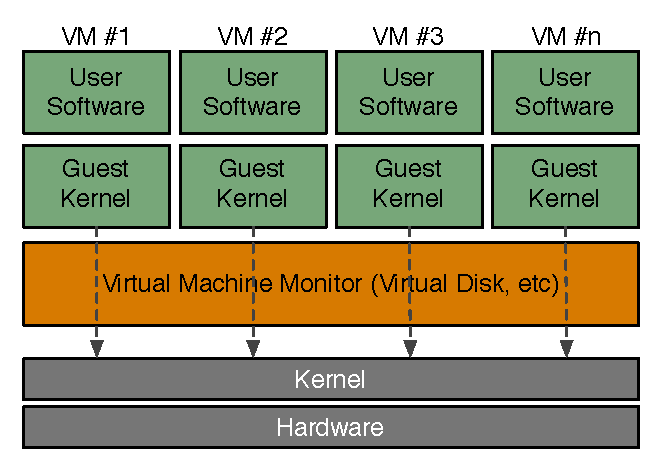
\includegraphics[scale=0.75]{intro/native-virtualization}
	\caption{Native Virtualization}
\end{figure}

Native virtualization leverages hardware-assisted capabilities available in the
latest processors from Intel (Intel VT) and Advanced Micro Devices (AMD-V) to
provide near-native performance. Prior to these processors, the x86
architecture did not meet some fundamental requirements for virtualization,
making it difficult to implement a virtual machine monitor for this type of
processor.

These requirements include: equivalence - a program running under the virtual
machine should exhibit a behavior essentially identical to the original
physical machine; resource control - the virtual machine must be in complete
control of the virtualized resources and efficiency - where the virtual machine
should not significantly degrade workload performance.~\cite{wp-native-virt}

\section{Para-virtualization}
\label{sec:intro:intro:para}

However, native virtualization may incur a performance penalty.  The VM monitor
must provide the VM with an image of an entire system, including virtual BIOS,
virtual memory space, and virtual devices. The VM monitor also must create and
maintain data structures for the virtual components, such as a shadow memory
page table. These data structures must be updated for every corresponding
access by the VMs.

\begin{figure}[H]
	\center
	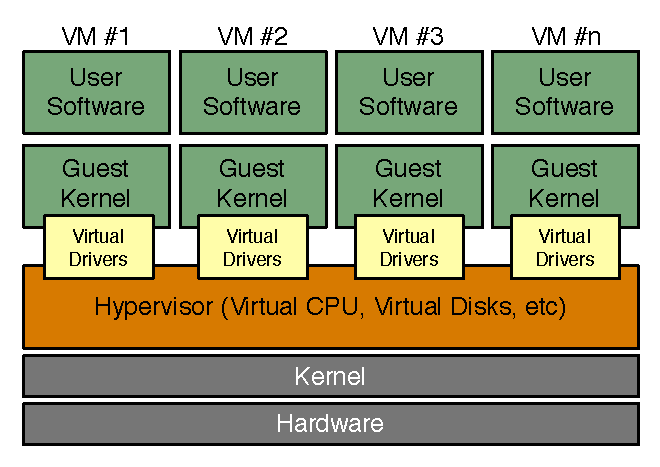
\includegraphics[scale=0.75]{intro/para-virtualization}
	\caption{Para-Virtualization}
\end{figure}

Therefore, para-virtualization exposes a virtual architecture that is slightly
different than the physical architecture. The differences in the architecture
are driven by improvements in scalability or reductions in system complexity.
Modifying the architecture breaks backwards compatibility with existing OS
code, which is a major disadvantage. However, it enables to co-design the
virtual architecture with the operating system, which gives a considerable
latitude when exploring issues of scale.

Para-virtualization has been used in previous VMMs, including VM/370 and Disco.
These systems added a combination of instructions, registers, or devices to the
virtual architecture to improve performance. However, because the goal of these
systems was to run legacy OSs, their use of para-virtualization was
minimized.~\cite{denali}

Porting an operating system to run on the VMM is similar to supporting a new
hardware platform, however the process is simplified because the para-virtual
machine architecture is very similar to the underlying native hardware.

The term ``para-virtualization'' was first used in the research literature in
association with the Denali virtual machine monitor~\cite{denali}. The term
is also used to describe the Xen, L4, Virtual, Iron and TRANGO hypervisors. All
these projects use paravirtualization techniques to support high performance
virtual machines on x86 hardware.


\section{Operating System-Level Virtualization}
\label{sec:intro:intro:oslevel}

\textit{Operating System-Level Virtualization} is a server virtualization
technology which virtualizes servers on a operating system (kernel) layer. It
can be thought of as partitioning a single physical server into multiple small
computational partitions. Each such partition looks and feels like a real
server, from the point of view of its owner. On Unix systems, this technology
can be thought of as an advanced extension of the standard chroot mechanism.

\begin{figure}[H]
	\center
	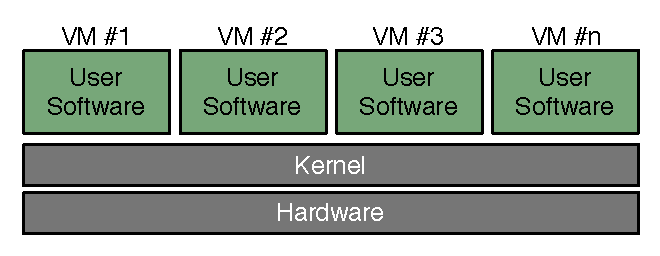
\includegraphics[scale=0.75]{intro/os-virtualization}
	\caption{Operating System-Level Virtualization}
\end{figure}

Many terms for the computational partitions exist and mostly depend on the
implementation: virtual environments (VE), virtual private servers (VPS),
jails, guests, zones, vservers, containers, etc.

The operating system level architecture has low overhead that helps to maximize
efficient use of server resources. Due to a single-kernel approach, this type
of virtualization introduces only a negligible overhead and allows running
hundreds of virtual private servers on a single physical server. In contrast,
approaches such as emulation and para-virtualization cannot achieve such level
of density, due to overhead of running multiple kernels. On the other hand,
operating system-level virtualization does not allow running different
operating systems (i.e. different kernels), although different libraries,
distributions etc. are possible.~\cite{wp-os-virt}

\chapter{The Linux-VServer Project}

The Linux-VServer project implements operating system-level virtualization
based on \textit{Security Contexts} which permit the creation of many
independent \textit{Virtual Private Servers} (VPS) that run simultaneously on a
single physical server at full speed, efficiently sharing hardware resources.

A VPS provides an almost identical operating environment as a conventional
Linux server. All services, such as ssh, mail, web and databases, can be
started on such a VPS, without (or in special cases with only minimal)
modification, just like on any real server.

Each virtual server has its own user account database and root password and is
isolated from other virtual servers, except for the fact that they share the
same hardware resources.


\section{Rationale}

Over the years, computers have become sufficiently powerful to use
virtualization to create the illusion of many smaller virtual machines, each
running a separate operating system instance.

There are several kinds of \textit{Virtual Machines} (VMs) providing similar
features, but differ in the degree of abstraction and the methods used for
virtualization.

Most of them accomplish what they do by emulating some real or fictional
hardware, which in turn consume real resources from the \textit{Host} (the
machine running the VMs). This approach, used by most system emulators, allows
the emulator to run an arbitrary operating systems, even for a different
hardware architecture. No modifications need to be made to the \textit{Guest}
(the operating system running in the VM) because it isn't aware of the fact
that it isn't running on real hardware.

Some system emulators require small modifications or specialized drivers to be
added to Host or Guest to improve performance and minimize the overhead
required for hardware emulation. Although this significantly improves
efficiency, there are still large amounts of resources being wasted in caches
and mediation between Guest and Host.

But suppose you do not want to run many different operating systems
simultaneously on a single box. Most applications running on a server do not
require hardware access or kernel level code, and could easily share a machine
with others, if they could be separated and secured...


\section{The Concept}

At a basic level, a Linux server consists of three building blocks: hardware,
kernel and applications. The hardware usually depends on the provider or system
maintainer, and, while it has a big influence on the overall performance, it
cannot be changed that easily, and will likely differ from one setup to
another.

The main purpose of the kernel is to build an abstraction layer on top of the
hardware to allow processes (applications) to work with and operate on
resources without knowing the details of the underlying hardware. Ideally,
those processes would be completely hardware agnostic, by being written in an
interpreted language and therefore not requiring any hardware-specific
knowledge.

Given that a system has enough resources to drive ten times the number of
applications a single Linux server would usually require, why not put ten
servers on that box, which will then share the available resources in an
efficient manner?

Most server applications (e.g. httpd) will assume that it is the only
application providing a particular service, and usually will also assume a
certain filesystem layout and environment. This dictates that similar or
identical services running on the same physical server, but for example, only
differing in their addresses, have to be coordinated. This typically requires a
great deal of administrative work which can lead to reduced system stability
and security.

The basic concept of the Linux-VServer solution is to separate the user-space
environment into distinct units (Virtual Private Servers) in such a way that
each VPS looks and feels like a real server to the processes contained within.

Although different Linux distributions use (sometimes heavily) patched kernels
to provide special support for unusual hardware or extra functionality, most
Linux distributions are not tied to a special kernel.

Linux-VServer uses this fact to allow several distributions, to be run
simultaneously on a single, shared kernel, without direct access to the
hardware, and share the resources in a very efficient way.


\section{Usage Scenarios}

The primary goal of this project is to create virtual servers sharing the same
machine. A virtual server operates like a normal Linux server. It runs normal
services such as telnet, mail servers, web servers, and database servers.


\subsection{Administrative Separation}

As the hardware evolves, it is tempting to put more and more tasks on a server.
Though Linux could reliably handle it, at some point, the system administrator
will likely end up with too much stuff and users on one system and worrying
about system updates. Additionally, separating different or similar services
which otherwise would interfere with each other, either because they are poorly
designed or because they are simply incapable of peaceful coexistence for
whatever reason, may often be complex or even impossible.

The Linux-VServer project addresses this issue. The same box is able to run
multiple virtual servers and each one does the job it is supposed to do. If the
administrator needs to upgrade to PHP 5 for a given project, he can update just
one virtual server and does not affect the others.

Also, the root password of a virtual servers can be given to foreign
administrators, thus allows him to perform updates, restart services or update
system configuration without having to know or worry about other virtual
servers hosted on the same machine. This allows a clever provider to sell
Virtual Private Servers, which uses less resources than other virtualization
techniques, which in turn allows to put more units on a single machine.

The list of providers doing so is relatively long, and so this is rightfully
considered the main area of application. See the Linux-VServer project
page\footnote{\url{http://linux-vserver.org/VServer_Hosting}} for a (possibly
incomplete) list of companies providing Virtual Private Servers based on the
Linux-VServer technology.


\subsection{Enhancing Security}

While it can be interesting to run several virtual servers in one box, there is
one concept potentially more generally useful. Imagine a physical server
running a single virtual server. The goal is to isolate the main environment
from any service, any network. You boot in the main environment, start very few
services and then continue in the virtual server.

The service in the main environment would be:

\begin{itemize}
	\item Unreachable from the network.

	\item Able to log messages from the virtual server in a secure way. The
		virtual server would be unable to change/erase the logs. Even a cracked
		virtual server would not be able the edit the log.

	\item Able to run intrusion detection facilities, potentially spying the
		state of the virtual server without being accessible or noticed. For
		example, tripwire could run there and it would be impossible to
		circumvent its operation or trick it.
\end{itemize}

Another option is to put the firewall in a virtual server, and pull in the DMZ,
containing each service in a separate VPS. On proper configuration, this setup
can reduce the number of required machines drastically, without impacting
performance.


\subsection{Resource Indepedence}

Since virtual servers are only guests on the hardware they are using, they are
not aware of the specifics: they do not contain disk configurations, kernels or
network configurations.

One key feature of a virtual server is the independence from the actual
hardware. Most hardware issues are irrelevant for a virtual server
installation.

The main server acts as a host and takes care of all the details. The virtual
server is just a client and ignores all the details. As such, the client can be
moved to another physical server with very few manipulations.

For example, to move the virtual server from one physical computer to another,
it sufficient to do the following:

\begin{itemize}
	\item shutdown the running virtual server
	\item copy it over to the other machine
	\item copy the configuration
	\item start the virtual server on the new machine
\end{itemize}

No adjustments to user setup, password database or hardware configuration are
required, as long as both machine architectures are binary compatible.

Thus, once a virtual server is using more resource than expected, the
administrator can easily move it to another machine without the need to worry
about configuration files for disk layout, network interfaces etc. A virtual
server is just a directory on the filesystem of host system.


\subsection{Distribution Independence}

People are often talking about their preferred distribution. Should one use
Fedora, Debian or something else? Should one give a spin to the latest and
greatest distribution just for the sake of it?

With virtual servers, the choice of a distribution is less important. When you
select a distribution, you expect it will do the following:

\begin{itemize}
	\item Good hardware support/detection
	\item Good package technology/updates
	\item Good package selection
	\item Reliable packages
\end{itemize}

The choice is important because every service running on a box will be using
the same distribution. Most distributions out there are good and reliable.
Still each one has its peculiarities and probably flaws. For example, one
distribution is doing a great job on security but is not delivering the latest
and greatest PHP. Now because you have decided to use this distribution for
some projects, using virtual servers does not prevent you from using another
distribution for other projects or even a second virtual server for existing
projects.


\subsection{Fail-over Scenarios}

Pushing the limit a little further, replication technology could be used to
keep an up-to-the-minute copy of the filesystem of a running virtual server.
This would permit a very fast fail-over if the running server goes offline for
whatever reason.

All the known methods to accomplish this, starting with network replication via
rsync, or drbd, via network devices, or shared disk arrays, to distributed
filesystems, can be utilized to reduce the down-time and improve overall
efficiency.


\subsection{Experimenting and Upgrading}

If the system administrator intends to upgrade a system to get new features or
security updates, he probably first wants to test new packages on a development
machine, before the production server can be updated. Under normal
circumstances, i.e. all test have been passed, the upgrade procedure will look
something like this:

\begin{itemize}
	\item Doing a backup of the server
	\item Perform all the upgrades and install the new applications
\end{itemize}

Two hours later something does not work as expected and -- to make it even
worse -- it works fine on the development machine. Every system administrator
has experienced this scenario at least once.

Another solution to this problem would be to install the new production server
on new hardware, but this is not always possible, due to lack of hardware or
the effort needed to clone an existing machine.

Using virtual servers, all this becomes very easy:

\begin{itemize}
	\item Stop the virtual server in production
	\item Make a copy of the virtual server
	\item Perform the upgrades in the new virtual server
\end{itemize}

To get back to the example from above, two hours later something does not work
as expected and there is no immediate fix for the problem.

Again, using virtual servers, the (temporary) solution to this problem is very
easy:

\begin{itemize}
	\item Stop the new virtual server and assign it a new IP address
	\item Start both the old and new virtual server
\end{itemize}

Now the old one is still online and the issue can be tracked down on your new
virtual server using a different IP address. After the problem has been fixed
the new virtual server will be reassign the old IP address and serve for
production.


% TODO: more info needed here
\subsection{Development and Testing}

Consider a software tool or package which should be built for several versions
of a specific distribution (Mandrake 8.2, 9.0, 9.1, 9.2, 10.0) or even for
different distributions.

This is easily solved with Linux-VServer. Given plenty of disk space, the
different distributions can be installed and running side by side, simplifying
the task of switching from one to another.

Of course this can be accomplished by chroot() alone, but with Linux-VServer
it's a much more realistic simulation.


% TODO: more info needed here
\section{History}

\textbf{Jacques Gélinas} created the VServer project a number of years back.
He still does vserver development and the community can be glad to have him.
He's a genius, without him, Linux-VServer would not exist. Three cheers for
Jack.

But sometime during 2003 it became apparent that Jack didn't have the time to
keep vserver development up to pace. So in November, \textbf{Herbert Pötzl}
officially took charge of development. He now releases the vserver kernel
patches, announcing them on the vserver mailing list and making them available
for the public.

Additionally, \textbf{Enrico Scholz} decided to reimplement Jack's vserver
tools in \textbf{C}.  These are now distributed as util-vserver. They are
backward compatible to Jack's tools as far as possible, but follow the kernel
patch development more closely.

In 2005, \textbf{Benedikt Böhm} started another reimplementation of the
userspace utilities, although with a completely different architecture in mind.
This new implementation is known as VServer Control Daemon as you already may
know when you read this manual \texttt{;-)}

\chapter{Daemon Administration Methods}


% vcd.login
\section{vcd.login}

This method is used to authenticate against the user database. Internally it is
a no-op method, since every method call must be authenticated. This is only
usefull for GUIs or web panels, to let users login without actually doing
something.

\rpcsynopsisempty{vcd.login}

\begin{rpcaccess}
\rpcnocapability and \rpcnoownerchecks.
\end{rpcaccess}

\rpcreturnnil

\rpcnoerrors


% vcd.status
\section{vcd.status}

This method is used to retreive internal daemon statistics. The daemon stores a
lot of runtime information in VXDB that can be used by system administrators or
user to check the daemon or account healthiness respectively.

\rpcsynopsisempty{vcd.status}

\begin{rpcaccess}
\rpccapability{INFO} and \rpcnoownerchecks.
\end{rpcaccess}

\rpcreturnnil

\rpcnoerrors



% vcd.user.caps.add
\section{vcd.user.caps.add}

This method is used to add capabilities to the internal user database.

\begin{rpcsynopsis}{vcd.user.caps.add}{string username, string cap}
\rpcparam{username}{Unique username}
\rpcparam{cap}{Capability to add}
\end{rpcsynopsis}

\begin{rpcaccess}
\rpccapability{AUTH} and \rpcnoownerchecks.
\end{rpcaccess}

\rpcreturnnil

\rpcnoerrors


% vcd.user.caps.get
\section{vcd.user.caps.get}

This method is used to get information about configured capabilities in the
internal user database.

\begin{rpcsynopsis}{vcd.user.caps.get}{string username}
\rpcparam{username}{Unique username}
\end{rpcsynopsis}

\begin{rpcaccess}
\rpccapability{AUTH} and \rpcnoownerchecks.
\end{rpcaccess}

\rpcreturnsimple{an \texttt{array} of \texttt{string}s - on for each
	capability - }

\rpcnoerrors


% vcd.user.caps.remove
\section{vcd.user.caps.remove}

This method is used to remove information about configured capabilities from
the internal user database.

\begin{rpcsynopsis}{vcd.user.caps.remove}{string username, string cap}
\rpcparam{username}{Unique username}
\rpcparam{cap}{Capability to remove}
\end{rpcsynopsis}

\begin{rpcaccess}
\rpccapability{AUTH} and \rpcnoownerchecks.
\end{rpcaccess}

\rpcreturnnil

\rpcnoerrors


% vcd.user.get
\section{vcd.user.get}

This method is used to get information about configured users in the internal
user database.

\begin{rpcsynopsis}{vcd.user.get}{string username}
\rpcparam{username}{Unique username}
\end{rpcsynopsis}

\begin{rpcaccess}
\rpccapability{AUTH} and \rpcnoownerchecks.
\end{rpcaccess}

\begin{rpcreturncomplex}{\texttt{struct}}{string password, bool admin}
\rpcreturnparam{password}{Password hash for the specified user}
\rpcreturnparam{admin}{Set the administrator flag for the specified user}
\end{rpcreturncomplex}


% vcd.user.remove
\section{vcd.user.remove}

This method is used to remove information about configured users from the
internal user database.

\begin{rpcsynopsis}{vcd.user.remove}{string username}
\rpcparam{username}{Unique username}
\end{rpcsynopsis}

\begin{rpcaccess}
\rpccapability{AUTH} and \rpcnoownerchecks.
\end{rpcaccess}

\rpcreturnnil

\rpcnoerrors


% vcd.user.set
\section{vcd.user.set}

This method is used to set (add \& change) information about configured users
in the internal user database.

\begin{rpcsynopsis}{vcd.user.set}{string username, string password,
	bool admin}
\rpcparam{username}{Unique username}
\rpcparam{password}{Password for the specified user (if user already exists
	this value may be empty to not change the password)}
\rpcparam{admin}{Set the administrator flag for the specified user}
\end{rpcsynopsis}

\begin{rpcaccess}
\rpccapability{AUTH} and \rpcnoownerchecks.
\end{rpcaccess}

\rpcreturnnil

\rpcnoerrors




\part{Installation}

\part{Configuration and Maintenance}

\part{Command Reference}
\chapter{VServer Control Client}
\label{ch:cmdref:vcc}

\chapter{Daemon Administration Methods}


% vcd.login
\section{vcd.login}

This method is used to authenticate against the user database. Internally it is
a no-op method, since every method call must be authenticated. This is only
usefull for GUIs or web panels, to let users login without actually doing
something.

\rpcsynopsisempty{vcd.login}

\begin{rpcaccess}
\rpcnocapability and \rpcnoownerchecks.
\end{rpcaccess}

\rpcreturnnil

\rpcnoerrors


% vcd.status
\section{vcd.status}

This method is used to retreive internal daemon statistics. The daemon stores a
lot of runtime information in VXDB that can be used by system administrators or
user to check the daemon or account healthiness respectively.

\rpcsynopsisempty{vcd.status}

\begin{rpcaccess}
\rpccapability{INFO} and \rpcnoownerchecks.
\end{rpcaccess}

\rpcreturnnil

\rpcnoerrors



% vcd.user.caps.add
\section{vcd.user.caps.add}

This method is used to add capabilities to the internal user database.

\begin{rpcsynopsis}{vcd.user.caps.add}{string username, string cap}
\rpcparam{username}{Unique username}
\rpcparam{cap}{Capability to add}
\end{rpcsynopsis}

\begin{rpcaccess}
\rpccapability{AUTH} and \rpcnoownerchecks.
\end{rpcaccess}

\rpcreturnnil

\rpcnoerrors


% vcd.user.caps.get
\section{vcd.user.caps.get}

This method is used to get information about configured capabilities in the
internal user database.

\begin{rpcsynopsis}{vcd.user.caps.get}{string username}
\rpcparam{username}{Unique username}
\end{rpcsynopsis}

\begin{rpcaccess}
\rpccapability{AUTH} and \rpcnoownerchecks.
\end{rpcaccess}

\rpcreturnsimple{an \texttt{array} of \texttt{string}s - on for each
	capability - }

\rpcnoerrors


% vcd.user.caps.remove
\section{vcd.user.caps.remove}

This method is used to remove information about configured capabilities from
the internal user database.

\begin{rpcsynopsis}{vcd.user.caps.remove}{string username, string cap}
\rpcparam{username}{Unique username}
\rpcparam{cap}{Capability to remove}
\end{rpcsynopsis}

\begin{rpcaccess}
\rpccapability{AUTH} and \rpcnoownerchecks.
\end{rpcaccess}

\rpcreturnnil

\rpcnoerrors


% vcd.user.get
\section{vcd.user.get}

This method is used to get information about configured users in the internal
user database.

\begin{rpcsynopsis}{vcd.user.get}{string username}
\rpcparam{username}{Unique username}
\end{rpcsynopsis}

\begin{rpcaccess}
\rpccapability{AUTH} and \rpcnoownerchecks.
\end{rpcaccess}

\begin{rpcreturncomplex}{\texttt{struct}}{string password, bool admin}
\rpcreturnparam{password}{Password hash for the specified user}
\rpcreturnparam{admin}{Set the administrator flag for the specified user}
\end{rpcreturncomplex}


% vcd.user.remove
\section{vcd.user.remove}

This method is used to remove information about configured users from the
internal user database.

\begin{rpcsynopsis}{vcd.user.remove}{string username}
\rpcparam{username}{Unique username}
\end{rpcsynopsis}

\begin{rpcaccess}
\rpccapability{AUTH} and \rpcnoownerchecks.
\end{rpcaccess}

\rpcreturnnil

\rpcnoerrors


% vcd.user.set
\section{vcd.user.set}

This method is used to set (add \& change) information about configured users
in the internal user database.

\begin{rpcsynopsis}{vcd.user.set}{string username, string password,
	bool admin}
\rpcparam{username}{Unique username}
\rpcparam{password}{Password for the specified user (if user already exists
	this value may be empty to not change the password)}
\rpcparam{admin}{Set the administrator flag for the specified user}
\end{rpcsynopsis}

\begin{rpcaccess}
\rpccapability{AUTH} and \rpcnoownerchecks.
\end{rpcaccess}

\rpcreturnnil

\rpcnoerrors



\chapter{VServer Control Daemon Administration Tool}

\chapter{VServer Configuration Editor}
\label{ch:cmdref:vce}

\chapter{VServer Kernel Helper}
\label{ch:cmdref:vshelper}


\part{XML-RPC Method Reference}
% LaTeX commands used in the method reference

% synopsis
\newcommand{\rpcsynopsisempty}[1]{
	\subsection*{Synopsis}

	\begin{quote}
	\texttt{#1()}
	\end{quote}
}

\newenvironment{rpcsynopsis}[2]{
	\subsection*{Synopsis}

	\begin{quote}
	\texttt{#1(#2)}
	\end{quote}

	\begin{labeling}{000000000}
}{
	\end{labeling}
}

\newcommand{\rpcparam}[2]{\labelingitem{#1}{#2}}

% access restrictions
\newenvironment{rpcaccess}[0]{
	\subsection*{Access Restrictions}
}{}

\newcommand{\rpccapability}[1]{This method requires the \texttt{#1} capability}
\newcommand{\rpcnocapability}[0]{This method requires no capabilities }
\newcommand{\rpcownerchecks}[0]{needs to pass owner checks}
\newcommand{\rpcnoownerchecks}[0]{does not need to pass owner checks}

% return value
\newcommand{\rpcreturnnil}[0]{
	\subsection*{Return Value}

	On success \texttt{NIL} is returned, on error a fault notification is
	returned.
}

\newcommand{\rpcreturnsimple}[1]{
	\subsection*{Return Value}

	On success #1 is returned, on error a fault notification is returned.
}


\newenvironment{rpcreturncomplex}[2]{
	\subsection*{Return Value}

	On success #1 with the following signature is returned, on error a fault
	notification is returned.

	\begin{quote}
	\texttt{\{#2\}}
	\end{quote}

	\begin{labeling}{000000000}
}{
	\end{labeling}
}

\newcommand{\rpcreturnparam}[2]{\labelingitem{#1}{#2}}

% errors
\newcommand{\rpcnoerrors}[0]{
	\subsection*{Errors}

	This method does not return any errors beside the generic method errors.
}

\newenvironment{rpcerrors}[0]{
	\subsection*{Errors}

	Beside the generic method errors, this method may return the following
	specific errors:

	\begin{labeling}{000000000}
}{
	\end{labeling}
}

\newcommand{\rpcerror}[2]{\labelingitem{#1}{#2}}

\chapter{Introduction to virtualization}
\label{ch:intro:intro}


\section{What is virtualization?}
\label{sec:intro:intro:whatis}

Today, virtualization is a broad term that refers to the abstraction computer
resources. It has been widely used since the 1960s or earlier, and has been
applied to many different aspects and scopes of computing — from entire
computer systems to individual capabilities or components. The common theme of
all virtualization technologies is the hiding of technical detail.

\begin{quote}
Virtualization is, at its foundation, a technique for hiding the physical
characteristics of computing resources from the way in which other systems,
applications, or end users interact with those resources. This includes making
a single physical resource (such as a server, an operating system, an
application, or storage device) appear to function as multiple logical
resources; or it can include making multiple physical resources (such as
storage devices or servers) appear as a single logical resource.~\cite{ema101}
\end{quote}

\begin{center}
\rule{10.0em}{0.02em}
\end{center}

\begin{quote}
Virtualization is a framework or methodology of dividing the resources of a
computer into multiple execution environments, by applying one or more concepts
or technologies such as hardware and software partitioning, time-sharing,
partial or complete machine simulation, emulation, quality of service, and many
others.~\cite{singh-intro}
\end{quote}

\begin{center}
\rule{10.0em}{0.02em}
\end{center}

\begin{quote}
Virtualization is an abstraction layer that decouples the physical hardware
from the operating system to deliver greater IT resource utilization and
flexibility.

Virtualization allows multiple virtual machines, with heterogeneous operating
systems to run in isolation, side-by-side on the same physical machine. Each
virtual machine has its own set of virtual hardware (e.g., RAM, CPU, NIC, etc.)
upon which an operating system and applications are loaded. The operating
system sees a consistent, normalized set of hardware regardless of the actual
physical hardware components.~\cite{vmware-intro}
\end{quote}

Due to the abstract nature of these definitions the list of virtualization
types, implementations and frameworks is rather huge, and we trust that readers
will appreciate that this subject cannot be covered in great detail here.
Nevertheless the following list encompasses some popular virtualization
techniques, to give the reader -- at least -- a rough understanding of key
differences between current major technologies.

A rather complete list of virtualization frameworks can be found on Amit Singhs
page \textit{An Introduction to Virtualization}.~\cite{singh-intro}


\section{Simulation}
\label{sec:intro:intro:simulation}

A \textit{computer simulation} is an attempt to model a real-life situation on
a computer so that it can be studied to see how the system works. By changing
variables, predictions may be made about the behaviour of the system.

An interesting application of computer simulation is to simulate computers
using computers. The related software is called computer architecture
simulators, which can be further divided into instruction set simulators or
full system simulators.

An instruction set simulator is often provided with a debugger in order for a
software engineer to debug the program prior to obtaining target hardware.  GDB
is one of debuggers which have compiled-in ISS. It is sometimes integrated with
simulated peripheral circuits such as timers, interrupts, serial port, general
I/O port, etc to mimic the behavior of microcontroller.~\cite{wp-iss}


\section{Emulation}
\label{sec:intro:intro:emulation}

A \textit{Software Emulator} allows computer programs to run on a platform
(computer architecture and/or operating system) other than the one for which
they were originally written. More generally, emulation refers to the ability
of a program or device to imitate another program or device.

Many printers, for example, are designed to emulate Hewlett-Packard LaserJet
printers because so much software is written for HP printers. By emulating an
HP printer, a printer can work with any software written for a real HP printer.
Emulation tricks the software into believing that a device is really some other
device.

Another  popular use of emulators is to mimic the experience of running arcade
games or console games on personal computers. Emulating these on modern desktop
computers is usually less cumbersome and more reliable than relying on the
original machines, which are often old and hard to find, let alone repair.
Emulation of arcade and console systems on home PCs usually includes the
practice of illegally downloading software from various electronic distribution
sources.

In a theoretical sense, the Church-Turing thesis~\cite{church-turing}
implies that any operating environment can be emulated within any other. In
practice, however, it can be quite difficult, particularly when the exact
behavior of the system to be emulated is not documented and has to be deduced
through reverse engineering. It also says nothing about timing constraints --
if the emulator does not perform as quickly as the original hardware, the
emulated software may run much more slowly than it would have on the original
hardware.


\section{Simulation vs. Emulation}
\label{sec:intro:intro:simvsemu}

There is a lot of confusion between emulators and simulators, in fact, the
distinction between those two is not always easy to tell. Ed
Thelen~\cite{emu-vs-simu} has collected some opinions on the difference, some of
which are quoted below.

In October 2005, Peter Hans van den Muijzenberg wrote:

\begin{verbatim}
Hi,

Regarding the difference between simulation and emulation:
Not limited to computers I use this distinction:
- A simulation mimics the outward appearance
- An emulation mimics the cause/process.

If you want to convince people that watching television gives you
stomach-aches, you can simulate this by holding your chest/abdomen and
moan. You can emulate it by eating a kilo of unripe apples.

BFN,
                                Peter Hans van den Muijzenberg
\end{verbatim}

Another, quite theoretical view of the problem, from Arun Parajuli, January
2006:

\begin{verbatim}
In my view the difference between simulation and emulation is:

Emulation: A system X is said to emulate another system Y if the
behaviour of X is exactly the same as that of Y (same out put for
same input under similar conditions) but the mechanism to arrive at
the output (from the input) is different.  Emulation is generally
used when we don't exactly know the internal mechanism of the
original system but are familiar with the input/output pattern. For
example, neural networks may be used to emulate different systems.
Neural networks are trained to produce the same output for the same
input as that of the original system though the mechanism/procedure
to generate the output are quite different.

Simulation: A system X is said to simulate another system Y
when the internal mechanism/procedures of X is a mathematical
(or any other) model known to best represent the actual mechanism
of Y. Simulation is generally used when we have some mathematical
models of the original system (Y) and want to know output for a
given set of inputs. For example we may have a good mathematical
model of effect of water temperature on the hurricane formation. We
use that system to predict the nature of hurricanes for different
water temperatures. It is to be noted that the result of simulation
can sometimes be unverifiable. For example the hurricane pattern
suggested by the simulator for water temperature equal to 50 degree
Celsius will be difficult to verify because we may never encounter
such situation.

Arun Parajuli
\end{verbatim}


\section{Native Virtualization}
\label{sec:intro:intro:native}

Native virtualization, in which the Virtual Machine simulates complete hardware
to allow operation of an umodified operating system for the same type of CPU to
execute within the virtual machine container in complete isolation.

\begin{figure}[H]
	\center
	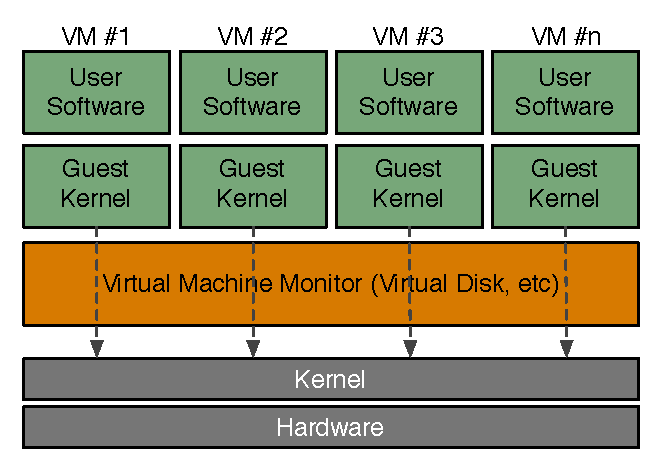
\includegraphics[scale=0.75]{intro/native-virtualization}
	\caption{Native Virtualization}
\end{figure}

Native virtualization leverages hardware-assisted capabilities available in the
latest processors from Intel (Intel VT) and Advanced Micro Devices (AMD-V) to
provide near-native performance. Prior to these processors, the x86
architecture did not meet some fundamental requirements for virtualization,
making it difficult to implement a virtual machine monitor for this type of
processor.

These requirements include: equivalence - a program running under the virtual
machine should exhibit a behavior essentially identical to the original
physical machine; resource control - the virtual machine must be in complete
control of the virtualized resources and efficiency - where the virtual machine
should not significantly degrade workload performance.~\cite{wp-native-virt}

\section{Para-virtualization}
\label{sec:intro:intro:para}

However, native virtualization may incur a performance penalty.  The VM monitor
must provide the VM with an image of an entire system, including virtual BIOS,
virtual memory space, and virtual devices. The VM monitor also must create and
maintain data structures for the virtual components, such as a shadow memory
page table. These data structures must be updated for every corresponding
access by the VMs.

\begin{figure}[H]
	\center
	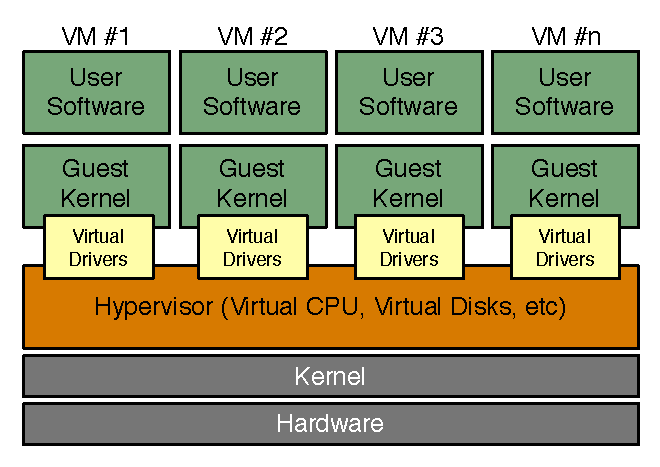
\includegraphics[scale=0.75]{intro/para-virtualization}
	\caption{Para-Virtualization}
\end{figure}

Therefore, para-virtualization exposes a virtual architecture that is slightly
different than the physical architecture. The differences in the architecture
are driven by improvements in scalability or reductions in system complexity.
Modifying the architecture breaks backwards compatibility with existing OS
code, which is a major disadvantage. However, it enables to co-design the
virtual architecture with the operating system, which gives a considerable
latitude when exploring issues of scale.

Para-virtualization has been used in previous VMMs, including VM/370 and Disco.
These systems added a combination of instructions, registers, or devices to the
virtual architecture to improve performance. However, because the goal of these
systems was to run legacy OSs, their use of para-virtualization was
minimized.~\cite{denali}

Porting an operating system to run on the VMM is similar to supporting a new
hardware platform, however the process is simplified because the para-virtual
machine architecture is very similar to the underlying native hardware.

The term ``para-virtualization'' was first used in the research literature in
association with the Denali virtual machine monitor~\cite{denali}. The term
is also used to describe the Xen, L4, Virtual, Iron and TRANGO hypervisors. All
these projects use paravirtualization techniques to support high performance
virtual machines on x86 hardware.


\section{Operating System-Level Virtualization}
\label{sec:intro:intro:oslevel}

\textit{Operating System-Level Virtualization} is a server virtualization
technology which virtualizes servers on a operating system (kernel) layer. It
can be thought of as partitioning a single physical server into multiple small
computational partitions. Each such partition looks and feels like a real
server, from the point of view of its owner. On Unix systems, this technology
can be thought of as an advanced extension of the standard chroot mechanism.

\begin{figure}[H]
	\center
	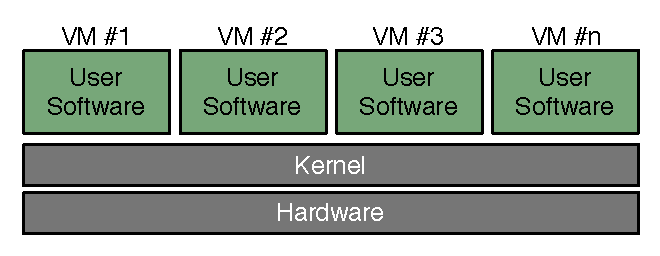
\includegraphics[scale=0.75]{intro/os-virtualization}
	\caption{Operating System-Level Virtualization}
\end{figure}

Many terms for the computational partitions exist and mostly depend on the
implementation: virtual environments (VE), virtual private servers (VPS),
jails, guests, zones, vservers, containers, etc.

The operating system level architecture has low overhead that helps to maximize
efficient use of server resources. Due to a single-kernel approach, this type
of virtualization introduces only a negligible overhead and allows running
hundreds of virtual private servers on a single physical server. In contrast,
approaches such as emulation and para-virtualization cannot achieve such level
of density, due to overhead of running multiple kernels. On the other hand,
operating system-level virtualization does not allow running different
operating systems (i.e. different kernels), although different libraries,
distributions etc. are possible.~\cite{wp-os-virt}

\chapter{Helper Methods}
\label{ch:rpcref:helper}


% helper.netup
\section{helper.netup}

This method is used to setup necessary network configuration during startup of
virtual servers. It is called by \texttt{vshelper} once the kernel has created
the network context. This method is not supposed to be called by a user or
administrator.

\begin{rpcsynopsis}{helper.netup}{int xid}
\rpcparam{xid}{Unique context ID}
\end{rpcsynopsis}

\begin{rpcaccess}
\rpccapability{HELPER} and \rpcnoownerchecks.
\end{rpcaccess}

\rpcreturnnil

\rpcnoerrors


% helper.restart
\section{helper.restart}

This method is used to remember reboot requests from vitrtual servers. It is
called by \texttt{vshelper} once virtual servers have issued a reboot system
call. After the request has been stored in VXDB the kernel terminates all
processes belonging to the virtual server, and calls \texttt{helper.shutdown}
afterwards.  This method is not supposed to be called by a user or
administrator.

\begin{rpcsynopsis}{helper.restart}{int xid}
\rpcparam{xid}{Unique context ID}
\end{rpcsynopsis}

\begin{rpcaccess}
\rpccapability{HELPER} and \rpcnoownerchecks.
\end{rpcaccess}

\rpcreturnnil

\rpcnoerrors


% helper.shutdown
\section{helper.shutdown}

This method is used to cleanup state data after virtual server shutdown. If a
reboot request has been recorded in VXDB by \texttt{helper.restart} the virtual
server is started again. This method is not supposed to be called by a user or
administrator.

\begin{rpcsynopsis}{helper.shutdown}{int xid}
\rpcparam{xid}{Unique context ID}
\end{rpcsynopsis}

\begin{rpcaccess}
\rpccapability{HELPER} and \rpcnoownerchecks.
\end{rpcaccess}

\rpcreturnnil

\rpcnoerrors



% helper.startup
\section{helper.startup}

This method is used to setup necessary configuration during startup. This
includes all configuration except network configuration, which is handled in
\texttt{helper.netup}. % FIXME: cross-ref to explanation of startup procedure

\begin{rpcsynopsis}{helper.startup}{int xid}
\rpcparam{xid}{Unique context ID}
\end{rpcsynopsis}

\begin{rpcaccess}
\rpccapability{HELPER} and \rpcnoownerchecks.
\end{rpcaccess}

\rpcreturnnil

\rpcnoerrors

\chapter{Daemon Administration Methods}


% vcd.login
\section{vcd.login}

This method is used to authenticate against the user database. Internally it is
a no-op method, since every method call must be authenticated. This is only
usefull for GUIs or web panels, to let users login without actually doing
something.

\rpcsynopsisempty{vcd.login}

\begin{rpcaccess}
\rpcnocapability and \rpcnoownerchecks.
\end{rpcaccess}

\rpcreturnnil

\rpcnoerrors


% vcd.status
\section{vcd.status}

This method is used to retreive internal daemon statistics. The daemon stores a
lot of runtime information in VXDB that can be used by system administrators or
user to check the daemon or account healthiness respectively.

\rpcsynopsisempty{vcd.status}

\begin{rpcaccess}
\rpccapability{INFO} and \rpcnoownerchecks.
\end{rpcaccess}

\rpcreturnnil

\rpcnoerrors



% vcd.user.caps.add
\section{vcd.user.caps.add}

This method is used to add capabilities to the internal user database.

\begin{rpcsynopsis}{vcd.user.caps.add}{string username, string cap}
\rpcparam{username}{Unique username}
\rpcparam{cap}{Capability to add}
\end{rpcsynopsis}

\begin{rpcaccess}
\rpccapability{AUTH} and \rpcnoownerchecks.
\end{rpcaccess}

\rpcreturnnil

\rpcnoerrors


% vcd.user.caps.get
\section{vcd.user.caps.get}

This method is used to get information about configured capabilities in the
internal user database.

\begin{rpcsynopsis}{vcd.user.caps.get}{string username}
\rpcparam{username}{Unique username}
\end{rpcsynopsis}

\begin{rpcaccess}
\rpccapability{AUTH} and \rpcnoownerchecks.
\end{rpcaccess}

\rpcreturnsimple{an \texttt{array} of \texttt{string}s - on for each
	capability - }

\rpcnoerrors


% vcd.user.caps.remove
\section{vcd.user.caps.remove}

This method is used to remove information about configured capabilities from
the internal user database.

\begin{rpcsynopsis}{vcd.user.caps.remove}{string username, string cap}
\rpcparam{username}{Unique username}
\rpcparam{cap}{Capability to remove}
\end{rpcsynopsis}

\begin{rpcaccess}
\rpccapability{AUTH} and \rpcnoownerchecks.
\end{rpcaccess}

\rpcreturnnil

\rpcnoerrors


% vcd.user.get
\section{vcd.user.get}

This method is used to get information about configured users in the internal
user database.

\begin{rpcsynopsis}{vcd.user.get}{string username}
\rpcparam{username}{Unique username}
\end{rpcsynopsis}

\begin{rpcaccess}
\rpccapability{AUTH} and \rpcnoownerchecks.
\end{rpcaccess}

\begin{rpcreturncomplex}{\texttt{struct}}{string password, bool admin}
\rpcreturnparam{password}{Password hash for the specified user}
\rpcreturnparam{admin}{Set the administrator flag for the specified user}
\end{rpcreturncomplex}


% vcd.user.remove
\section{vcd.user.remove}

This method is used to remove information about configured users from the
internal user database.

\begin{rpcsynopsis}{vcd.user.remove}{string username}
\rpcparam{username}{Unique username}
\end{rpcsynopsis}

\begin{rpcaccess}
\rpccapability{AUTH} and \rpcnoownerchecks.
\end{rpcaccess}

\rpcreturnnil

\rpcnoerrors


% vcd.user.set
\section{vcd.user.set}

This method is used to set (add \& change) information about configured users
in the internal user database.

\begin{rpcsynopsis}{vcd.user.set}{string username, string password,
	bool admin}
\rpcparam{username}{Unique username}
\rpcparam{password}{Password for the specified user (if user already exists
	this value may be empty to not change the password)}
\rpcparam{admin}{Set the administrator flag for the specified user}
\end{rpcsynopsis}

\begin{rpcaccess}
\rpccapability{AUTH} and \rpcnoownerchecks.
\end{rpcaccess}

\rpcreturnnil

\rpcnoerrors



\chapter{General Maintenance Methods}

The vx family of functions provide general maintenance facilities for virtual
servers.


% vx.create
\section{vx.create}

This method is used to create a new virtual server using a template cache.

\begin{rpcsynopsis}{vx.create}{string name, string template,
	bool force, bool copy, string vdir}
\rpcparam{name}{Unique name to use for the new virtual server}
\rpcparam{template}{Name of the template cache to use for the new virtual
	server}
\rpcparam{rebuild}{If the virtual server already exists and this is set to
	true a recursive unlink is performed before the template extraction
	takes place}
\end{rpcsynopsis}

\begin{rpcaccess}
\rpccapability{CREATE} and \rpcownerchecks. % FIXME: talk about this in intro
\end{rpcaccess}

\rpcreturnnil

\begin{rpcerrors}
\rpcerror{MEINVAL}{An empty template cache name was supplied, or the supplied
	value contained invalid characters}
\rpcerror{MEEXIST}{The virtual server already exists and the rebuild parameter
	was not set to true}
\rpcerror{MERUNNING}{The virtual server already exists, the rebuild parameter
	was set to true, but the existing virtual server is still running}
\end{rpcerrors}


% vx.exec
\section{vx.exec}

This method is used to execute a simple command inside a virtual server. This
method does not support redirection, pipes and other shell stuff, the command
line is executed with a plain \texttt{execvp}.

\begin{rpcsynopsis}{vx.exec}{string name, string command}
\rpcparam{name}{Unique virtual server name}
\rpcparam{command}{Simple command line to execute}
\end{rpcsynopsis}

\begin{rpcaccess}
\rpccapability{EXEC} and \rpcownerchecks.
\end{rpcaccess}

\rpcreturnsimple{a combined string of \texttt{STDOUT} and \texttt{STDERR}}

\begin{rpcerrors}
\rpcerror{MESTOPPED}{The specified virtual server is currently not running,
	therefore the command cannot be executed}
\end{rpcerrors}


% vx.kill
\section{vx.kill}

This method is used to send signals to processes inside a virtual server.

\begin{rpcsynopsis}{vx.kill}{string name, int pid, int sig}
\rpcparam{name}{Unique virtual server name}
\rpcparam{pid}{Process ID to send signal to, there are two special cases:\\
	0 = send signal to all processes\\
	1 = send signal to the real pid of a faked init}
\rpcparam{sig}{Signal Number, see the \texttt{signal(7)} man page for more
	information}
\end{rpcsynopsis}

\begin{rpcaccess}
\rpccapability{INIT} and \rpcownerchecks.
\end{rpcaccess}

\rpcreturnnil

\begin{rpcerrors}
\rpcerror{MESTOPPED}{The specified virtual server is currently not running,
	therefore no signals can be sent}
\end{rpcerrors}


% vx.reboot
\section{vx.reboot}

This method is used as a wrapper to vx.exec using the configured
\texttt{reboot} command.

\begin{rpcsynopsis}{vx.reboot}{string name}
\rpcparam{name}{Unique virtual server name}
\end{rpcsynopsis}

\begin{rpcaccess}
\rpccapability{INIT} and \rpcownerchecks.
\end{rpcaccess}

\rpcreturnsimple{the return value of \texttt{vx.exec}}

\begin{rpcerrors}
\rpcerror{MESTOPPED}{The specified virtual server is currently not running,
	therefore it cannot be stopped}
\end{rpcerrors}


% vx.remove
\section{vx.remove}

This method is used to remove a virtual server from the configuration database
and filesystem.

\begin{rpcsynopsis}{vx.remove}{string name}
\rpcparam{name}{Unique virtual server name}
\end{rpcsynopsis}

\begin{rpcaccess}
\rpccapability{CREATE} and \rpcownerchecks.
\end{rpcaccess}

\rpcreturnnil

\begin{rpcerrors}
\rpcerror{MERUNNING}{The specified virtual server is currently running,
	therefore it cannot be removed}
\rpcerror{MEEXIST}{The root filesystem fo the virtual server still exists after
	removal and no mount point exists for it. Manual check is needed.}
\end{rpcerrors}


% vx.rename
\section{vx.rename}

This method is used to rename a virtual server in the configuration database and
filesystem.

\begin{rpcsynopsis}{vx.rename}{string name, string newname}
\rpcparam{name}{Unique virtual server name}
\rpcparam{newname}{New unique virtual server name}
\end{rpcsynopsis}

\begin{rpcaccess}
\rpccapability{CREATE} and \rpcownerchecks.
\end{rpcaccess}

\rpcreturnnil

\begin{rpcerrors}
\rpcerror{MERUNNING}{The specified virtual server is currently running,
	therefore it cannot be renamed}
\rpcerror{MEEXIST}{The specified new virtual server name currently exists and
	cannot be used}
\end{rpcerrors}


% vx.start
\section{vx.start}

This method is used to start a virtual server.

\begin{rpcsynopsis}{vx.start}{string name}
\rpcparam{name}{Unique virtual server name}
\end{rpcsynopsis}

\begin{rpcaccess}
\rpccapability{INIT} and \rpcownerchecks.
\end{rpcaccess}

\rpcreturnnil

\begin{rpcerrors}
\rpcerror{MERUNNING}{The specified virtual server is currently running,
	therefore it cannot be started again}
\end{rpcerrors}


% vx.status
\section{vx.status}

This method is used to obtain status information about a virtual server.

\begin{rpcsynopsis}{vx.status}{string name}
\rpcparam{name}{Unique virtual server name}
\end{rpcsynopsis}

\begin{rpcaccess}
\rpccapability{INIT} and \rpcownerchecks.
\end{rpcaccess}

\begin{rpcreturncomplex}{\texttt{struct}}{bool running}
\rpcreturnparam{running}{This value is set to true if the specified virtual
	server is currently running, false otherwise}
\end{rpcreturncomplex}

\rpcnoerrors


% vx.stop
\section{vx.stop}

This method is used as a wrapper to vx.exec using the configured \texttt{halt}
command.

\begin{rpcsynopsis}{vx.stop}{string name}
\rpcparam{name}{Unique virtual server name}
\end{rpcsynopsis}

\begin{rpcaccess}
\rpccapability{INIT} and \rpcownerchecks.
\end{rpcaccess}

\rpcreturnsimple{the return value of \texttt{vx.exec}}

\begin{rpcerrors}
\rpcerror{MESTOPPED}{The specified virtual server is currently not running,
	therefore it cannot be stopped}
\end{rpcerrors}

\chapter{Database Manipulation Methods}
\label{ch:rpcref:vxdb}

The \texttt{vxdb} family of functions provide manipulation facilities for the
configuration database.


% vxdb.dx.limit.get
\section{vxdb.dx.limit.get}

This method is used to get information about configured disk limits.

\begin{rpcsynopsis}{vxdb.dx.limit.get}{string name}
\rpcparam{name}{Unique virtual server name}
\end{rpcsynopsis}

\begin{rpcaccess}
\rpccapability{DLIM} and \rpcownerchecks.
\end{rpcaccess}

\begin{rpcreturncomplex}{a \texttt{struct}}{uint32 space, uint32 inodes,
	int reserved}
\rpcreturnparam{space}{Maximum amount of disk space for this virtual server
	in KB}
\rpcreturnparam{inodes}{Maximum number of inodes for this virtual server}
\rpcreturnparam{reserved}{Disk space reserved for the super-user (root)
	\emph{inside} the virtual server in percent}
\end{rpcreturncomplex}

\rpcnoerrors


% vxdb.dx.limit.remove
\section{vxdb.dx.limit.remove}

This method is used to remove information about configured disk limits.

\begin{rpcsynopsis}{vxdb.dx.limit.remove}{string name}
\rpcparam{name}{Unique virtual server name}
\end{rpcsynopsis}

\begin{rpcaccess}
\rpccapability{DLIM} and \rpcownerchecks.
\end{rpcaccess}

\rpcreturnnil

\rpcnoerrors


% vxdb.dx.limit.set
\section{vxdb.dx.limit.set}

This method is used to set (add \& change) information about configured disk
limits.

\begin{rpcsynopsis}{vxdb.dx.limit.set}{string name, uint32 space,
	uint32 inodes, int reserved}
\rpcparam{name}{Unique virtual server name}
\rpcparam{space}{Maximum amount of disk space for this virtual server in KB}
\rpcparam{inodes}{Maximum number of inodes for this virtual server}
\rpcparam{reserved}{Disk space reserved for the super-user (root)
	\emph{inside} the virtual server in percent}
\end{rpcsynopsis}

\begin{rpcaccess}
\rpccapability{DLIM} and \rpcownerchecks.
\end{rpcaccess}

\rpcreturnnil

\rpcnoerrors


% vxdb.init.get
\section{vxdb.init.get}

This method is used to get information about configured \texttt{init},
\texttt{halt} and \texttt{reboot} commands.

\begin{rpcsynopsis}{vxdb.init.get}{string name}
\rpcparam{name}{Unique virtual server name}
\end{rpcsynopsis}

\begin{rpcaccess}
\rpccapability{INIT} and \rpcownerchecks.
\end{rpcaccess}

\begin{rpcreturncomplex}{a \texttt{struct}}{string init, string halt,
	string reboot}
\rpcreturnparam{init}{Absolute path of the init command \emph{inside} the
	virtual server (defaults to \texttt{/sbin/init} if empty)}
\rpcreturnparam{halt}{Absolute path of the halt command \emph{inside} the
	virtual server (defaults to \texttt{/sbin/halt} if empty)}
\rpcreturnparam{reboot}{Absolute path of the reboot command \emph{inside} the
	virtual server (defaults to \texttt{/sbin/reboot} if empty)}
\end{rpcreturncomplex}

\rpcnoerrors


% vxdb.init.set
\section{vxdb.init.set}

This method is used to set (change) information about configured \texttt{init},
\texttt{halt} and \texttt{reboot} commands.

\begin{rpcsynopsis}{vxdb.init.set}{string name, string init, string halt,
	string reboot}
\rpcparam{name}{Unique virtual server name}
\rpcparam{init}{Absolute path of the init command \emph{inside} the virtual
	server (defaults to \texttt{/sbin/init} if empty)}
\rpcparam{halt}{Absolute path of the halt command \emph{inside} the virtual
	server (defaults to \texttt{/sbin/halt} if empty)}
\rpcparam{reboot}{Absolute path of the reboot command \emph{inside} the
	virtual server (defaults to \texttt{/sbin/reboot} if empty)}
\end{rpcsynopsis}

\rpcreturnnil

\rpcnoerrors


% vxdb.list
\section{vxdb.list}

This method is used to get a list of all currently configured and owned virtual
servers.

\begin{rpcsynopsis}{vxdb.list}{string username}
\rpcparam{username}{Unique username (this value may be empty to return a list
containing all virtual servers)}
\end{rpcsynopsis}

\begin{rpcaccess}
\rpcnocapability and \rpcownerchecks. The owner checks do not check the usual
\texttt{name} parameter here, instead it returns all virtual servers that would
pass owner checks.
\end{rpcaccess}


\rpcreturnsimple{an \texttt{array} of \texttt{string}s -- one for each virtual
	server --}

\rpcnoerrors


% vxdb.mount.get
\section{vxdb.mount.get}

This method is used to get information about configured mount points.

\begin{rpcsynopsis}{vxdb.mount.get}{string name, string dst}
\rpcparam{name}{Unique virtual server name}
\rpcparam{dst}{Absolute destination path for the mount point inside the
	virtual server (this value may be empty to return a list of all
	configured mount points)}
\end{rpcsynopsis}

\begin{rpcaccess}
\rpccapability{MOUNT} and \rpcownerchecks.
\end{rpcaccess}

\begin{rpcreturncomplex}{an \texttt{array} of \texttt{struct}s -- one for each
	mount point --}{string src, string dst, string type, string opts}
\rpcreturnparam{src}{Absolute source path \emph{inside} the virtual server or
	arbitrary identifier (defaults to \texttt{none} if empty)}
\rpcreturnparam{dst}{Absolute destination path for the mount point inside the
	virtual server}
\rpcreturnparam{type}{Filesystem type for the specified source path
	(defaults to \texttt{auto}} if empty)
\rpcreturnparam{opts}{Mount options for the specified filesystem
	(defaults to \texttt{defaults} if empty)}
\end{rpcreturncomplex}

\rpcnoerrors


% vxdb.mount.remove
\section{vxdb.mount.remove}

This method is used to remove information about configured mount points.

\begin{rpcsynopsis}{vxdb.mount.remove}{string name, string dst}
\rpcparam{name}{Unique virtual server name}
\rpcparam{dst}{Absolute destination path for the mount point inside the
	virtual server (this value may be empty to remove all configured mount
	points)}
\end{rpcsynopsis}

\begin{rpcaccess}
\rpccapability{MOUNT} and \rpcownerchecks.
\end{rpcaccess}

\rpcreturnnil

\rpcnoerrors


% vxdb.mount.set
\section{vxdb.mount.set}

This method is used to set (add \& change) information about configured mount
points.

\begin{rpcsynopsis}{vxdb.mount.set}{string name, string src, string dst,
	string type, string opts}
\rpcparam{name}{Unique virtual server name}
\rpcparam{src}{Absolute source path \emph{inside} the virtual server or
	arbitrary identifier (defaults to \texttt{none} if empty)}
\rpcparam{dst}{Absolute destination path for the mount point inside the
	virtual server}
\rpcparam{type}{Filesystem type for the specified source path (defaults to
	\texttt{auto} if empty)}
\rpcparam{opts}{Mount options for the specified filesystem (defaults to
	\texttt{defaults} if empty)}
\end{rpcsynopsis}

\begin{rpcaccess}
\rpccapability{MOUNT} and \rpcownerchecks.
\end{rpcaccess}

\rpcreturnnil

\rpcnoerrors


% vxdb.name.get
\section{vxdb.name.get}

This method is used to lookup the name of a virtual server by its corresponding
context ID.

\begin{rpcsynopsis}{vxdb.name.get}{int xid}
\rpcparam{xid}{Unique context ID}
\end{rpcsynopsis}

\begin{rpcaccess}
% FIXME: INFO cap may expose information leak.
\rpccapability{INFO} and \rpcnoownerchecks.
\end{rpcaccess}

\rpcreturnsimple{a \texttt{string} containing the virtual server name}

\rpcnoerrors


% vxdb.nx.addr.get
\section{vxdb.nx.addr.get}

This method is used to get information about configured network addresses.

\begin{rpcsynopsis}{vxdb.nx.addr.get}{string name, string addr}
\rpcparam{name}{Unique virtual server name}
\rpcparam{addr}{Network address in dot-decimal form (this value may be empty
	to return a list of all configured network adresses)}
\end{rpcsynopsis}

\begin{rpcaccess}
\rpccapability{NET} and \rpcownerchecks.
\end{rpcaccess}

\begin{rpcreturncomplex}{an \texttt{array} of \texttt{struct}s -- one for each
	network address --}{string addr, string netmask}
\rpcreturnparam{addr}{Network address in dot-decimal form}
\rpcreturnparam{netmask}{Network mask in dot-decimal form (defaults to
	\texttt{255.255.255.0} if empty)}
\end{rpcreturncomplex}

\rpcnoerrors


% vxdb.nx.addr.remove
\section{vxdb.nx.addr.remove}

This method is used to remove information about configured network addresses.

\begin{rpcsynopsis}{vxdb.nx.addr.remove}{string name, string addr}
\rpcparam{name}{Unique virtual server name}
\rpcparam{addr}{Network address in dot-decimal form (this value may be empty to
	remove all configured network adresses)}
\end{rpcsynopsis}

\begin{rpcaccess}
\rpccapability{NET} and \rpcownerchecks.
\end{rpcaccess}

\rpcreturnnil

\rpcnoerrors


% vxdb.nx.addr.set
\section{vxdb.nx.addr.set}

This method is used to set (add \& change) information about configured network
addresses.

\begin{rpcsynopsis}{vxdb.nx.addr.set}{string name, string addr, string netmask}
\rpcparam{name}{Unique virtual server name}
\rpcparam{addr}{Network address in dot-decimal form}
\rpcparam{netmask}{Network mask in dot-decimal form (defaults to
	\texttt{255.255.255.0} if empty)}
\end{rpcsynopsis}

\begin{rpcaccess}
\rpccapability{NET} and \rpcownerchecks.
\end{rpcaccess}

\rpcreturnnil

\rpcnoerrors


% vxdb.nx.broadcast.get
\section{vxdb.nx.broadcast.get}

This method is used to get information about the configured broadcast address.

\begin{rpcsynopsis}{vxdb.nx.broadcast.get}{string name}
\rpcparam{name}{Unique virtual server name}
\end{rpcsynopsis}

\begin{rpcaccess}
\rpccapability{NET} and \rpcownerchecks.
\end{rpcaccess}

\rpcreturnsimple{a \texttt{string} containing the broadcast address}

\rpcnoerrors


% vxdb.nx.broadcast.remove
\section{vxdb.nx.broadcast.remove}

This method is used to remove information about the configured broadcast
address.

\begin{rpcsynopsis}{vxdb.nx.broadcast.remove}{string name}
\rpcparam{name}{Unique virtual server name}
\end{rpcsynopsis}

\begin{rpcaccess}
\rpccapability{NET} and \rpcownerchecks.
\end{rpcaccess}

\rpcreturnnil

\rpcnoerrors


% vxdb.vx.broadcast.set
\section{vxdb.nx.broadcast.set}

This method is used to set (change) information about the configured broadcast
address.

\begin{rpcsynopsis}{vxdb.nx.broadcast.set}{string name, string broadcast}
\rpcparam{name}{Unique virtual server name}
\rpcparam{broadcast}{Broadcast address in dot-decimal form}
\end{rpcsynopsis}

\begin{rpcaccess}
\rpccapability{NET} and \rpcownerchecks.
\end{rpcaccess}

\rpcreturnnil

\rpcnoerrors


% vxdb.owner.add
\section{vxdb.owner.add}

This method is used to add users to the list of configured owners in the
internal user database.

\begin{rpcsynopsis}{vxdb.owner.add}{string name, string username}
\rpcparam{name}{Unique virtual server name}
\rpcparam{username}{Unique username}
\end{rpcsynopsis}

\begin{rpcaccess}
\rpccapability{AUTH} and \rpcnoownerchecks.
\end{rpcaccess}

\rpcreturnnil

\rpcnoerrors


% vxdb.owner.get
\section{vxdb.owner.get}

This method is used to get information about configured owners in the internal
user database.

\begin{rpcsynopsis}{vxdb.owner.get}{string name}
\rpcparam{name}{Unique virtual server name}
\end{rpcsynopsis}

\begin{rpcaccess}
\rpccapability{AUTH} and \rpcnoownerchecks.
\end{rpcaccess}

\rpcreturnsimple{an \texttt{array} of \texttt{string}s -- one for each
	owner --}

\rpcnoerrors


% vxdb.owner.remove
\section{vxdb.owner.remove}

This method is used to remove information about configured owners from the
internal user database.

\begin{rpcsynopsis}{vxdb.owner.remove}{string name, string username}
\rpcparam{name}{Unique virtual server name}
\rpcparam{username}{Unique username (this value may be empty to remove all
	configured owners)}
\end{rpcsynopsis}

\begin{rpcaccess}
\rpccapability{AUTH} and \rpcnoownerchecks.
\end{rpcaccess}

\rpcreturnnil

\rpcnoerrors


% vxdb.vdir.get
\section{vxdb.vdir.get}

This method is used to get the absolute root filesystem path of a virtual
server.

\begin{rpcsynopsis}{vxdb.vdir.get}{string name}
\rpcparam{name}{Unique virtual server name}
\end{rpcsynopsis}

\begin{rpcaccess}
% FIXME: INFO cap may expose information leak.
\rpccapability{INFO} and \rpcnoownerchecks.
\end{rpcaccess}

\rpcreturnsimple{a \texttt{string} containing the absolute root filesystem
	path}

\rpcnoerrors


% vxdb.vx.bcaps.add
\section{vxdb.vx.bcaps.add}

This method is used to add information about configured system capabilities.

\begin{rpcsynopsis}{vxdb.vx.bcaps.add}{string name, string bcap}
\rpcparam{name}{Unique virtual server name}
\rpcparam{bcap}{System capability to add}
\end{rpcsynopsis}

\begin{rpcaccess}
\rpccapability{BCAP} and \rpcownerchecks.
\end{rpcaccess}

\rpcreturnnil

\rpcnoerrors


% vxdb.vx.bcaps.get
\section{vxdb.vx.bcaps.get}

This method is used to get information about configured system capabilities.

\begin{rpcsynopsis}{vxdb.vx.bcaps.get}{string name}
\rpcparam{name}{Unique virtual server name}
\end{rpcsynopsis}

\begin{rpcaccess}
\rpccapability{BCAP} and \rpcownerchecks.
\end{rpcaccess}

\rpcreturnsimple{an \texttt{array} of \texttt{string}s -- one for each system
	capability --}

\rpcnoerrors


% vxdb.vx.bcaps.remove
\section{vxdb.vx.bcaps.remove}

This method is used to remove information about configured system capabilities.

\begin{rpcsynopsis}{vxdb.vx.bcaps.remove}{string name, string bcap}
\rpcparam{name}{Unique virtual server name}
\rpcparam{bcap}{System capability to remove}
\end{rpcsynopsis}

\begin{rpcaccess}
\rpccapability{BCAP} and \rpcownerchecks.
\end{rpcaccess}

\rpcreturnnil

\rpcnoerrors


% vxdb.vx.ccaps.add
\section{vxdb.vx.ccaps.add}

This method is used to add information about configured context capabilities.

\begin{rpcsynopsis}{vxdb.vx.ccaps.add}{string name, string ccap}
\rpcparam{name}{Unique virtual server name}
\rpcparam{ccap}{Context capability to add}
\end{rpcsynopsis}

\begin{rpcaccess}
\rpccapability{CCAP} and \rpcownerchecks.
\end{rpcaccess}

\rpcreturnnil

\rpcnoerrors


% vxdb.vx.ccaps.get
\section{vxdb.vx.ccaps.get}

This method is used to get information about configured context capabilities.

\begin{rpcsynopsis}{vxdb.vx.ccaps.get}{string name}
\rpcparam{name}{Unique virtual server name}
\end{rpcsynopsis}

\begin{rpcaccess}
\rpccapability{CCAP} and \rpcownerchecks.
\end{rpcaccess}

\rpcreturnsimple{an \texttt{array} of \texttt{string}s -- one for each context
	capability --}

\rpcnoerrors


% vxdb.vx.ccaps.remove
\section{vxdb.vx.ccaps.remove}

This method is used to remove information about configured context
capabilities.

\begin{rpcsynopsis}{vxdb.vx.ccaps.remove}{string name, string ccap}
\rpcparam{name}{Unique virtual server name}
\rpcparam{ccap}{Context capability to remove}
\end{rpcsynopsis}

\begin{rpcaccess}
\rpccapability{CCAP} and \rpcownerchecks.
\end{rpcaccess}

\rpcreturnnil

\rpcnoerrors


% vxdb.vx.flags.add
\section{vxdb.vx.flags.add}

This method is used to add information about configured context flags.

\begin{rpcsynopsis}{vxdb.vx.flags.add}{string name, string flag}
\rpcparam{name}{Unique virtual server name}
\rpcparam{flag}{Context flag to add}
\end{rpcsynopsis}

\begin{rpcaccess}
\rpccapability{CFLAG} and \rpcownerchecks.
\end{rpcaccess}

\rpcreturnnil

\rpcnoerrors


% vxdb.vx.flags.get
\section{vxdb.vx.flags.get}

This method is used to get information about configured context flags.

\begin{rpcsynopsis}{vxdb.vx.flags.get}{string name}
\rpcparam{name}{Unique virtual server name}
\end{rpcsynopsis}

\begin{rpcaccess}
\rpccapability{CFLAG} and \rpcownerchecks.
\end{rpcaccess}

\rpcreturnsimple{an \texttt{array} of \texttt{string}s -- one for each context
	flag -- }

\rpcnoerrors


% vxdb.vx.flags.remove
\section{vxdb.vx.flags.remove}

This method is used to remove information about configured context flags.

\begin{rpcsynopsis}{vxdb.vx.flags.remove}{string name, string flag}
\rpcparam{name}{Unique virtual server name}
\rpcparam{flag}{Context flag to remove}
\end{rpcsynopsis}

\begin{rpcaccess}
\rpccapability{CFLAG} and \rpcownerchecks.
\end{rpcaccess}

\rpcreturnnil

\rpcnoerrors


% vxdb.vx.limit.get
\section{vxdb.vx.limit.get}

This method is used to get information about configured resource limits.

\begin{rpcsynopsis}{vxdb.vx.limit.get}{string name, string limit}
\rpcparam{name}{Unique virtual server name}
\rpcparam{limit}{Limit type to get (this value may be empty to retrieve all
	configured resource limits)}
\end{rpcsynopsis}

\begin{rpcaccess}
\rpccapability{RLIM} and \rpcownerchecks.
\end{rpcaccess}

\begin{rpcreturncomplex}{an \texttt{array} of \texttt{struct}s -- one for each
	resource limit --}{string limit, uint64 soft, uint64 max}
\rpcreturnparam{limit}{Limit type to add or change}
\rpcreturnparam{soft}{Softl imit for the specified type}
\rpcreturnparam{max}{Hard limit for the specified type}
\end{rpcreturncomplex}

\rpcnoerrors


% vxdb.vx.limit.remove
\section{vxdb.vx.limit.remove}

This method is used to remove information about configured resource limits.

\begin{rpcsynopsis}{vxdb.vx.limit.remove}{string name, string limit}
\rpcparam{name}{Unique virtual server name}
\rpcparam{limit}{Limit type to remove (this value may be empty to remove all
	configured resource limits)}
\end{rpcsynopsis}

\begin{rpcaccess}
\rpccapability{RLIM} and \rpcownerchecks.
\end{rpcaccess}

\rpcreturnnil

\rpcnoerrors


% vxdb.vx.limit.set
\section{vxdb.vx.limit.set}

This method is used to set (add \& change) information about configured
resource limits.

\begin{rpcsynopsis}{vxdb.vx.limit.set}{string name, string limit, uint64 soft,
	uint64 max}
\rpcparam{name}{Unique virtual server name}
\rpcparam{limit}{Limit type to add or change}
\rpcparam{soft}{Softl imit for the specified type}
\rpcparam{max}{Hard limit for the specified type}
\end{rpcsynopsis}

\begin{rpcaccess}
\rpccapability{RLIM} and \rpcownerchecks.
\end{rpcaccess}

\rpcreturnnil

\rpcnoerrors


% vxdb.vx.sched.get
\section{vxdb.vx.sched.get}

This method is used to get information about configured CPU scheduler buckets.

\begin{rpcsynopsis}{vxdb.vx.sched.get}{string name, int cpuid}
\rpcparam{name}{Unique virtual server name}
\rpcparam{cpuid}{CPU ID as listed in \texttt{/proc/cpuinfo}}
\end{rpcsynopsis}

\begin{rpcaccess}
\rpccapability{SCHED} and \rpcownerchecks.
\end{rpcaccess}

\begin{rpcreturncomplex}{an \texttt{array} of \texttt{struct}s -- one for each
	CPU ID --}{int cpuid, int interval, int fillrate, int interval2,
	int fillrate2, int tokensmin, int tokensmax}
\rpcreturnparam{cpuid}{CPU ID as listed in \texttt{/proc/cpuinfo}}
\rpcreturnparam{interval}{Interval between fills in jiffies}
\rpcreturnparam{fillrate}{Tokens to fill each interval}
\rpcreturnparam{interval2}{Interval between fills in jiffies (IDLE time
	setting)}
\rpcreturnparam{fillrate2}{Tokens to fill each interval (IDLE time setting)}
\rpcreturnparam{tokensmin}{Minimum number of tokens to schedule processes}
\rpcreturnparam{tokensmax}{Maximum number of tokens in the bucket}
\end{rpcreturncomplex}

\rpcnoerrors


% vxdb.vx.sched.remove
\section{vxdb.vx.sched.remove}

This method is used to remove information about configured CPU scheduler
buckets.

\begin{rpcsynopsis}{vxdb.vx.sched.remove}{string name, int cpuid}
\rpcparam{name}{Unique virtual server name}
\rpcparam{cpuid}{CPU ID as listed in \texttt{/proc/cpuinfo}}
\end{rpcsynopsis}

\begin{rpcaccess}
\rpccapability{SCHED} and \rpcownerchecks.
\end{rpcaccess}

\rpcreturnnil

\rpcnoerrors


% vxdb.vx.sched.set
\section{vxdb.vx.sched.set}

This method is used to set (add \& change) information about configured CPU
scheduler buckets.

\begin{rpcsynopsis}{vxdb.vx.sched.set}{string name, int cpuid, int interval,
	int fillrate, int interval2, int fillrate2, int tokensmin, int tokensmax}
\rpcparam{name}{Unique virtual server name}
\rpcparam{cpuid}{CPU ID as listed in \texttt{/proc/cpuinfo}}
\rpcparam{interval}{Interval between fills in jiffies}
\rpcparam{fillrate}{Tokens to fill each interval}
\rpcparam{interval2}{Interval between fills in jiffies (IDLE time setting)}
\rpcparam{fillrate2}{Tokens to fill each interval (IDLE time setting)}
\rpcparam{tokensmin}{Minimum number of tokens to schedule processes}
\rpcparam{tokensmax}{Maximum number of tokens in the bucket}
\end{rpcsynopsis}

\begin{rpcaccess}
\rpccapability{SCHED} and \rpcownerchecks.
\end{rpcaccess}

\rpcreturnnil

\rpcnoerrors


% vxdb.vx.uname.get
\section{vxdb.vx.uname.get}

This method is used to get information about configured virtual system
information.

\begin{rpcsynopsis}{vxdb.vx.uname.get}{string name, string uname}
\rpcparam{name}{Unique virtual server name}
\rpcparam{uname}{System information type (this value may be empty to retrieve
	information about all configured system information types)}
\end{rpcsynopsis}

\begin{rpcaccess}
\rpccapability{UNAME} and \rpcownerchecks.
\end{rpcaccess}

\begin{rpcreturncomplex}{an \texttt{array} of \texttt{struct}s -- one for each
	system information type --}{string uname, string value}
\rpcreturnparam{uname}{System information type}
\rpcreturnparam{value}{System information value}
\end{rpcreturncomplex}

\rpcnoerrors


% vxdb.vx.uname.remove
\section{vxdb.vx.uname.remove}

This method is used to remove information about configured virtual system
information.

\begin{rpcsynopsis}{vxdb.vx.uname.remove}{string name, string uname}
\rpcparam{name}{Unique virtual server name}
\rpcparam{uname}{System information type}
\end{rpcsynopsis}

\begin{rpcaccess}
\rpccapability{UNAME} and \rpcownerchecks.
\end{rpcaccess}

\rpcreturnnil

\rpcnoerrors


% vxdb.vx.uname.set
\section{vxdb.vx.uname.set}

This method is used to set (add \& change) information about configured virtual
system information.

\begin{rpcsynopsis}{vxdb.vx.uname.set}{string name, string uname, string value}
\rpcparam{name}{Unique virtual server name}
\rpcparam{uname}{System information type}
\rpcparam{value}{System information value to set}
\end{rpcsynopsis}

\begin{rpcaccess}
\rpccapability{UNAME} and \rpcownerchecks.
\end{rpcaccess}

\rpcreturnnil

\rpcnoerrors


% vxdb.xid.get
\section{vxdb.xid.get}

This method is used to lookup the Context ID of a virtual server by its name.

\begin{rpcsynopsis}{vxdb.xid.get}{string name}
\rpcparam{name}{Unique virtual server name}
\end{rpcsynopsis}

\begin{rpcaccess}
% FIXME: INFO cap may expose information leak.
\rpccapability{INFO} and \rpcnoownerchecks.
\end{rpcaccess}

\rpcreturnsimple{an \texttt{int} containing the Context ID of the specified
	virtual server}

\rpcnoerrors


\backmatter
\bibliography{manual}

\end{document}
